\section{Casi d'uso}
\subsection{Scopo}
Lo scopo di questa sezione è la descrizione in elenco di tutti i casi d'uso individuati dal gruppo, in riferimento alle funzionalità dell'applicazione.
\subsection{Attori}
Come accordato con il proponente, non essendo richiesto alcun servizio di autenticazione e tantomeno la figura di un amministratore per la gestione del database, è presente un solo attore nella gerarchia: l'utente generico.

\begin{figure}[h]
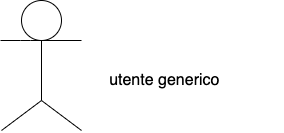
\includegraphics[width=1cm]{section/Images/Utente.png}
\centering
\caption{Gerarchia attori}
\end{figure}

\begin{description}
\item[Utente]:
Si riferisce all'utente generico che può accedere alla piattaforma e utilizzare tutti i servizi disponibili.
\end{description}

\newpage
\subsection{Elenco casi d'uso}
\subsubsection{UC1 - Caricamento del dataset}
\begin{figure}[h]
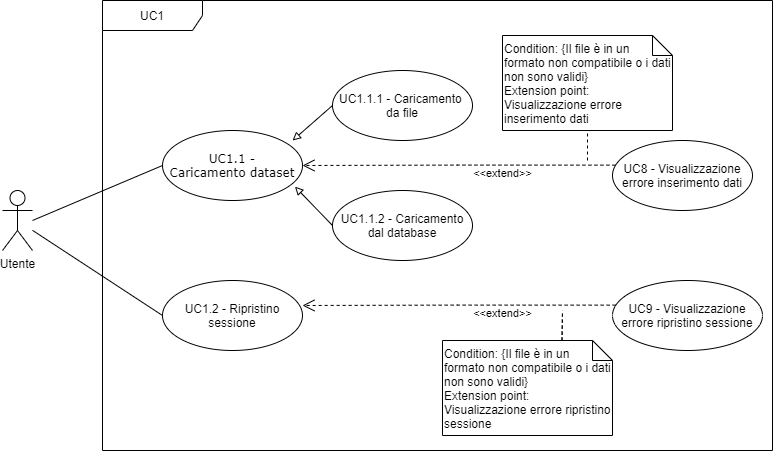
\includegraphics[width=\linewidth]{section/Images/UC1.png}
\centering
\caption{UC1 - Caricamento del dataset}
\end{figure}
\begin{itemize}
	\item \textbf{Attore primario}: Utente.
	\item \textbf{Precondizioni}: Il sistema è raggiungibile e funzionante.
	\item \textbf{Postcondizioni}: Viene visualizzato un messaggio che avvisa l'utente del corretto caricamento dei dati e della loro validità.
	\item \textbf{Scenario principale}:
		\begin{enumerate}
			\item L'utente accede al sistema;
			\item L'utente sceglie come ricavare i dati:
				\begin{enumerate}[(a)]
			\item L'utente seleziona la funzionalità "carica file" [UC1.1];
			\item L'utente seleziona un dataset tra quelli disponibili nel database [UC1.2].
				\end{enumerate}
		\end{enumerate}
	\item \textbf{Estensioni}:
	\begin{enumerate}[(a)]
		\item Nel caso in cui il file sia in un formato sbagliato o i dati non sono validi:
		\begin{enumerate}[1.]
			\item i dati non vengono caricati nel sistema;
			\item viene visualizzato un errore esplicativo [UC7].
		\end{enumerate}
	\end{enumerate}
\end{itemize}

\subsubsection{UC1.1 - Caricamento dataset da file}

\begin{itemize}
	\item \textbf{Attore primario}: Utente.
	\item \textbf{Precondizioni}: Il sistema è raggiungibile e funzionante. L'utente ha a disposizione un dataset in formato CSV.
	\item \textbf{Postcondizioni}: I dati presenti nel file vengono caricati nel sistema. Viene visualizzato un messaggio che avvisa l'utente del corretto caricamento e della validità dei dati.
	\item \textbf{Scenario principale}: L'utente sceglie di caricare un dataset personale o ricavato da altre fonti esterne.
	
\end{itemize}

\subsubsection{UC1.2 - Caricamento dataset dal database}

\begin{itemize}
	\item \textbf{Attore primario}: Utente.
	\item \textbf{Precondizioni}: Il sistema è raggiungibile e funzionante. L'utente effettua una query dal database disponibile per prelevare il dataset.
	\item \textbf{Postcondizioni}: I dati vengono caricati nel sistema. Viene visualizzato un messaggio che avvisa l'utente del corretto caricamento e della loro validità.
	\item \textbf{Scenario principale}: L'utente sceglie di caricare un dataset tra quelli presenti nel database.
	
\end{itemize}


  
\subsection{UC2 - Selezione delle dimensioni da utilizzare}
\begin{itemize}
	\item \textbf{Attore primario}: Utente;
	\item \textbf{Precondizioni}: L'utente ha caricato i dati nel sistema [UC1];
	\item \textbf{Postcondizioni}: Le dimensioni scelte vengono aggiornate nel sistema e i dati sono pronti per essere visualizzati [UC6];
	\item \textbf{Scenario principale}:
		\begin{enumerate}
			\item All'utente viene presentata una schermata con tutte le dimensioni presenti nel dataset caricato già selezionate di default;
			\item Per ogni dimensione è presente una cella da selezionare nel caso la si voglia utilizzare o meno;
			\item L'utente seleziona le dimensioni che desidera analizzare.
		\end{enumerate}
	\item \textbf{Estensioni:}
		\begin{enumerate}[(a)]
			\item Nel caso in cui l'utente non abbia selezionato nessuna dimensione:
			\begin{enumerate}[1.]
				\item Le dimensioni non vengono aggiornate nel sistema;
				\item Viene visualizzato un messaggio d'errore esplicativo [UC12].
			\end{enumerate}
		\end{enumerate}
\end{itemize}
\subsection{UC5 - Scelta della \glo{visualizzazione}}
\begin{figure}[h]
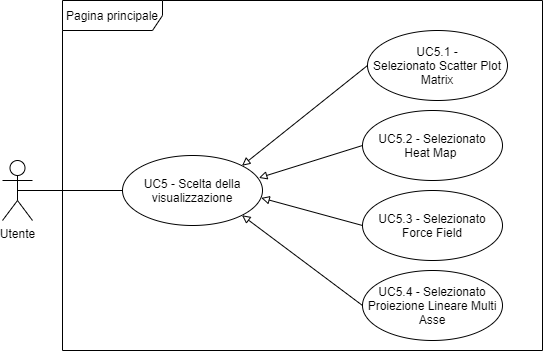
\includegraphics[width=\linewidth]{Section/Images/UC5.png}
\centering
\caption{UC5 - Scelta della visualizzazione}
\end{figure}
\begin{itemize}
	\item \textbf{Attore primario}: Utente;
	\item \textbf{Precondizioni}: L'utente ha caricato dei dati nel sistema e ha selezionato le dimensioni da utilizzare [UC2].
	\item \textbf{Postcondizioni}: Viene mostrata la visualizzazione scelta, con possibilità di personalizzazione [UC6]. La scelta viene salvata nel sistema.
	\item \textbf{Scenario principale}: L'utente seleziona la visualizzazione che vuole utilizzare tra quelle disponibili.
	\item \textbf{Generalizzazioni}: L'utente seleziona una delle seguenti opzioni:
		\begin{enumerate}
			\item \glo{\textit{Scatter Plot Matrix}} [UC5.1];
			\item \glo{\textit{Heat Map}} [UC5.2];
			\item \glo{\textit{Force Field}} [UC5.3];
			\item \glo{\textit{Proiezione Lineare Multi Asse}} [UC5.4].
		\end{enumerate}

\end{itemize}
\subsubsection{UC5.1 - Selezionato Scatter Plot Matrix}
\begin{itemize}
	\item \textbf{Attore primario}: Utente.
	\item \textbf{Precondizioni}: L'utente ha caricato dei dati nel sistema [UC1] e ha selezionato le dimensioni da utilizzare [UC2].
	\item \textbf{Postcondizioni}: Viene mostrata la visualizzazione \glo{\textit{Scatter Plot Matrix}} scelta dall'utente, con possibilità di personalizzazione.
	\item \textbf{Scenario principale}: L'utente seleziona la visualizzazione \glo{\textit{Scatter Plot Matrix}} e il sistema ritorna un grafico con cui si può interagire.
\end{itemize}
\subsubsection{UC5.2 - Selezionato Heat Map}
\begin{itemize}
	\item \textbf{Attore primario}: Utente.
	\item \textbf{Precondizioni}: L'utente ha caricato dei dati nel sistema e ha selezionato le dimensioni da utilizzare [UC2].
	\item \textbf{Postcondizioni}: Viene mostrata la visualizzazione \glo{\textit{Heat Map}} scelta dall'utente, con possibilità di personalizzazione.
	\item \textbf{Scenario principale}: L'utente seleziona la visualizzazione \glo{\textit{Heat Map}} e il sistema ritorna un grafico con cui si può interagire.

\end{itemize}
\subsubsection{UC5.3 Scelta visualizzazione Force Field}
\begin{figure}[h]
\centering
\caption{}
\end{figure}
\begin{itemize}
	\item \textbf{Attore primario}: Utente.
	\item \textbf{Precondizioni}:
	\item \textbf{Postcondizioni}:
	\item \textbf{Scenario principale}:
		\begin{enumerate}
			\item L'utente seleziona la visualizzazione Force Field
		\end{enumerate}
	\item \textbf{Estensioni}:
	\begin{enumerate}[(a)]
		\item Nel caso in cui non è stato caricato alcun dato o non è stata scelta alcuna dimensione:
		\begin{enumerate}[1.]
			\item il grafico non viene visualizzato;
			\item viene visualizzato un errore esplicativo [UCx.3].
		\end{enumerate}
	\end{enumerate}
\end{itemize}
\subsubsection{UC5.4 - Selezionato Proiezione Lineare Multi Asse}

\begin{itemize}
	\item \textbf{Attore primario}: Utente.
	\item \textbf{Precondizioni}: L'utente ha caricato dei dati nel sistema e ha selezionato le dimensioni da utilizzare.
	\item \textbf{Postcondizioni}: Viene mostrata la visualizzazione \glo{\textit{Proiezione Lineare Multi Asse}} scelta dall'utente, con possibilità di personalizzazione [UC6.4].
	\item \textbf{Scenario principale}: L'utente seleziona la visualizzazione \glo{\textit{Proiezione Lineare Multi Asse}} e il sistema ritorna un grafico con cui si può interagire.
\end{itemize}
\subsubsection{UC7 - Salva sessione}
\begin{itemize}
	\item \textbf{Attore primario}: Utente.
	\item \textbf{Precondizioni}: L'utente ha caricato dei dati nel sistema [UC1] e ha scelto il tipo di grafico da visualizzare [UC5]
	\item \textbf{Postcondizioni}: L'utente possiede un file \glo{JSON} per il ripristino della sessione.
	\item \textbf{Scenario principale}:
		\begin{enumerate}
			\item L'utente ha una sessione di lavoro aperta.
			\item L'utente seleziona la funzionalità "salva sessione";
			\item L'utente seleziona la directory in cui salvare il file.
		\end{enumerate}
\end{itemize}
\subsection{UC8 - Personalizzazione Force Field}
\begin{itemize}
	\item \textbf{Attore primario}: Utente.
	
	\item \textbf{Precondizioni}: L'utente ha scelto il grafico \textit{Force Field} [UC5.3].
	
	\item \textbf{Postcondizioni}: Il grafico viene aggiornato.
	
	\item \textbf{Scenario principale}: L'utente visualizza:
	
\begin{enumerate}
	\item Una lista con le funzioni di forza fornite dal sistema e può scegliere quale utilizzare tra quelle disponibili; 
	\item Una lista con tutte i tipi di distanza disponibili nel sistema e può scegliere quale utilizzare per il calcolo. 
\end{enumerate}	
	Inoltre l'utente può decidere alcuni stili del grafico, tra cui:
		\begin{enumerate}
			\item Scegliere quale dimensione utilizzare per il colore dei punti nel grafico;
				
			\item Scegliere quale dimensione utilizzare per la forma dei punti nel grafico;
			
			\item Scegliere quale dimensione utilizzare per l'etichetta dei punti nel grafico;
			
			\item Scegliere quale dimensione utilizzare per la dimensione dei punti nel grafico;
				
		\end{enumerate}
		
	\item \textbf{Estensioni}:
	\begin{enumerate}[(a)]
		\item ...
	\end{enumerate}
\end{itemize}

